\chapter{Теория}
\section{Схема модели (каналы и накопители)}

Схема модели в виде каналов и накопителей представленна на рисунке \ref{s2}.

\begin{figure}[h]
	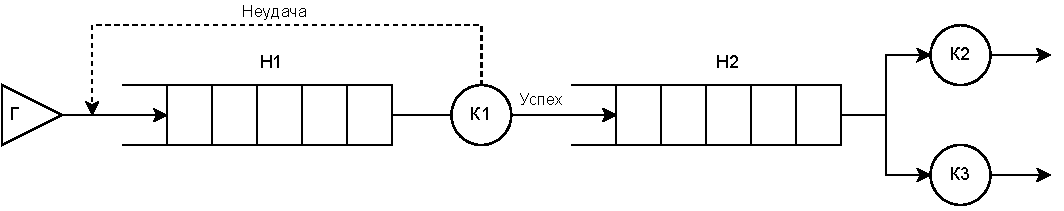
\includegraphics[width=1\linewidth]{"inc/img/Каналы и накопители.drawio.pdf"}
	\caption{Схема модели (каналы и накопители)}
	\label{s2}
\end{figure}

Согласно условию время прохождения нормконтроля и защиты НИР студентом подчиняется закону равномерного распределения. Автоматы обслуживания в модели классифицируются следующим образом:
\begin{itemize}
	\item К1 симулирует работу нормконтроля;
	\item К2 и К3 симулируют работу комиссий.
\end{itemize}

Эндогенные переменные -- время прохождения нормконтроля, вероятность успешного прохождения нормконтроля, время защиты НИР и вероятность успешной защиты $i$-ой комиссии ($i = \overline{0;1}$).

Экзогенные переменные -- $n_0$ равное числу защитившихся студентов и $n_1$ равное числу несдавших студентов.

Уравнения модели: вероятность сдачи $= n_0/(n_0+n_1)$

За единицу дискретного времени выбрана 0.01 минуты.
